\documentclass{beamer}

\usepackage{graphicx}
\usepackage{tikz}
\usepackage{amsmath}
\usepackage{amssymb}
\usepackage{booktabs}
\usepackage{comment}
\usepackage{hyperref}
\usepackage[absolute,overlay]{textpos}

\usetheme{Madrid}
\usecolortheme{default}

\title{Neutrinos: From Massless Ghosts in SM\\ to Oscillations, Masses and Beyond}
\author{Meihui Huang}
\date{June 2026}

\begin{document}

\frame{\titlepage}

% =================================================
\begin{frame}{Motivation}
\begin{itemize}
  \item Among the most abundant particles in the universe.
  \item In the Standard Model: assumed massless.
  \item Experiments show they oscillate flavors $\Rightarrow$ have mass.
  \item \textbf{First confirmed evidence for physics beyond the Standard Model}.
\end{itemize}

\vspace{0.4cm}
\centering
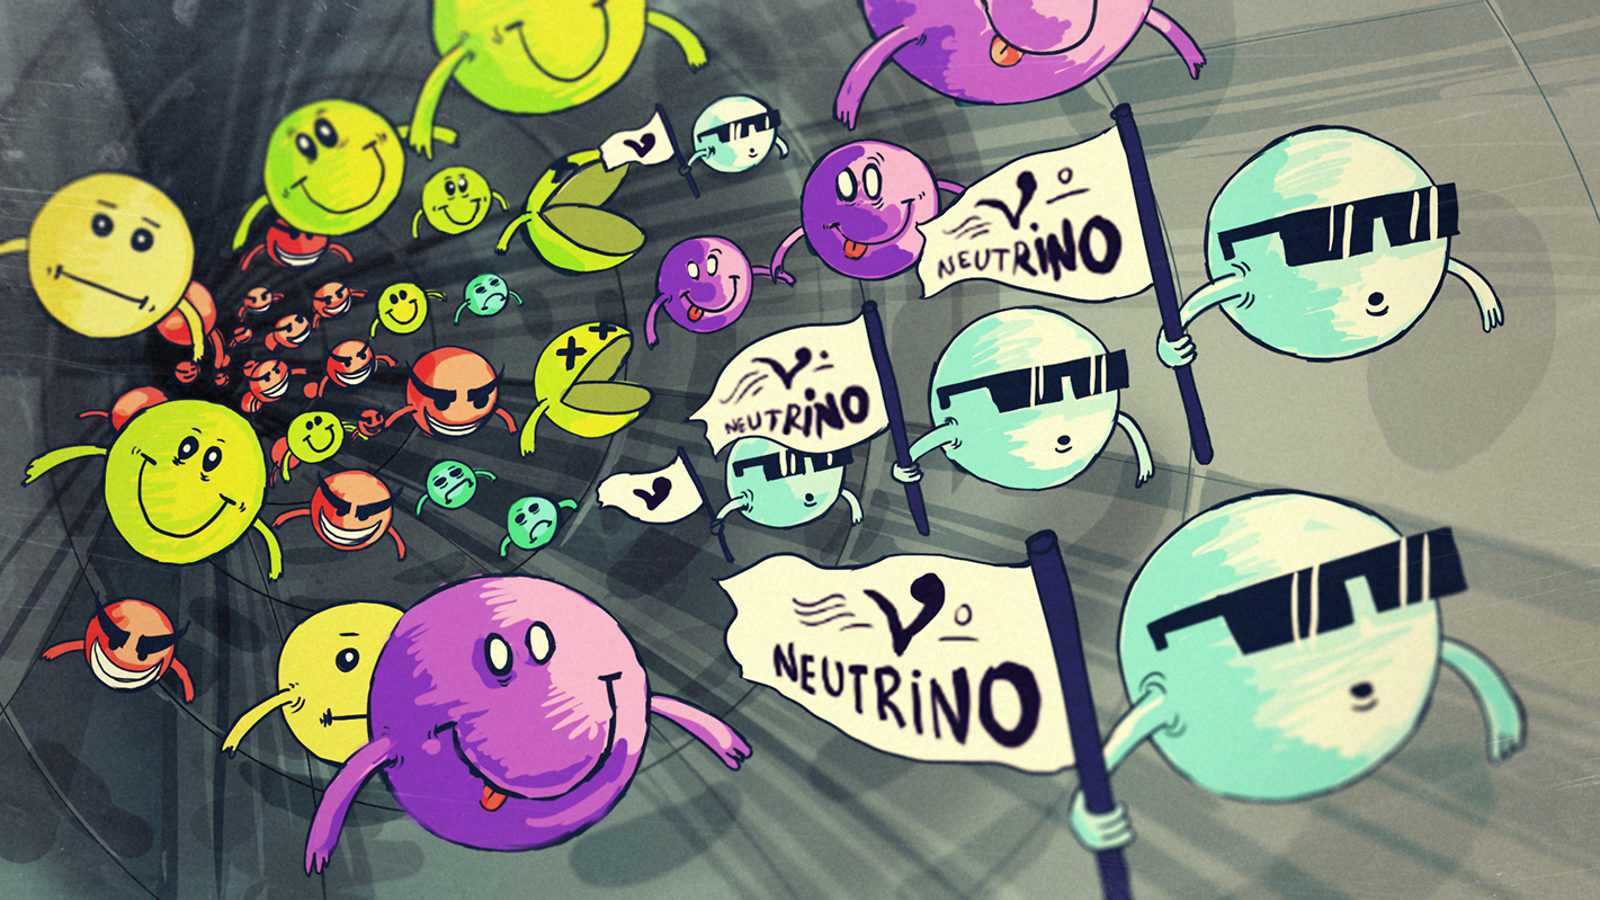
\includegraphics[height=4.5cm]{../figures/neutrinos_header.jpg}
\end{frame}

% =================================================
\begin{frame}{Outline}
\tableofcontents
\end{frame}

% =================================================
\section{Historical and Conceptual Origin}

% =================================================
\begin{frame}{The Beta Decay Puzzle}
\begin{itemize}
  \item Continuous electron spectrum in $\beta$-decay violates energy conservation?
  \item 1930: Pauli postulates a neutral, penetrating particle: the "neutron".
  \item 1934: Fermi develops weak interaction theory incorporating neutrinos.
\end{itemize}

\vspace{0.5cm}
\centering
\begin{columns}
    \column{0.5\textwidth}
    \centering
    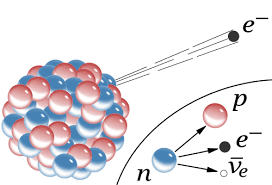
\includegraphics[height=3.5cm]{../figures/beta.png}

    \column{0.5\textwidth}
    \centering
    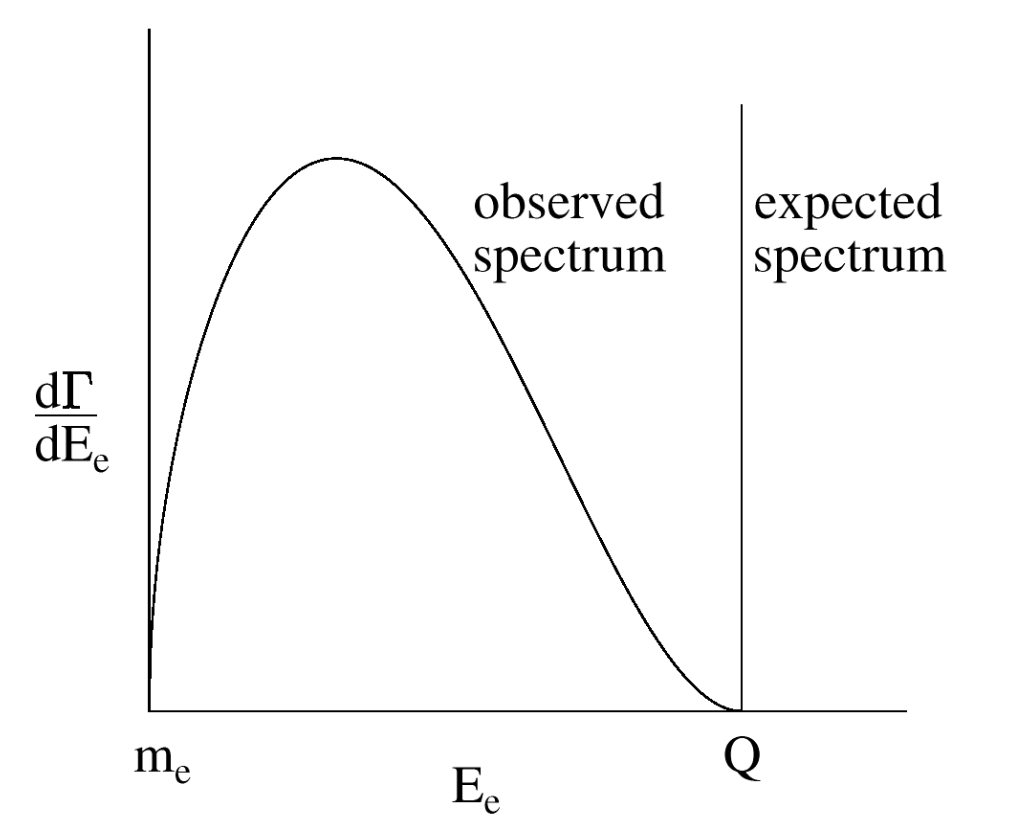
\includegraphics[height=4.5cm]{../figures/beta_energy_spectrum.png}
\end{columns}
\end{frame}

% =================================================
\begin{frame}{Fermi's Theory}
\vspace{0.5cm}
\centering
    \centering
    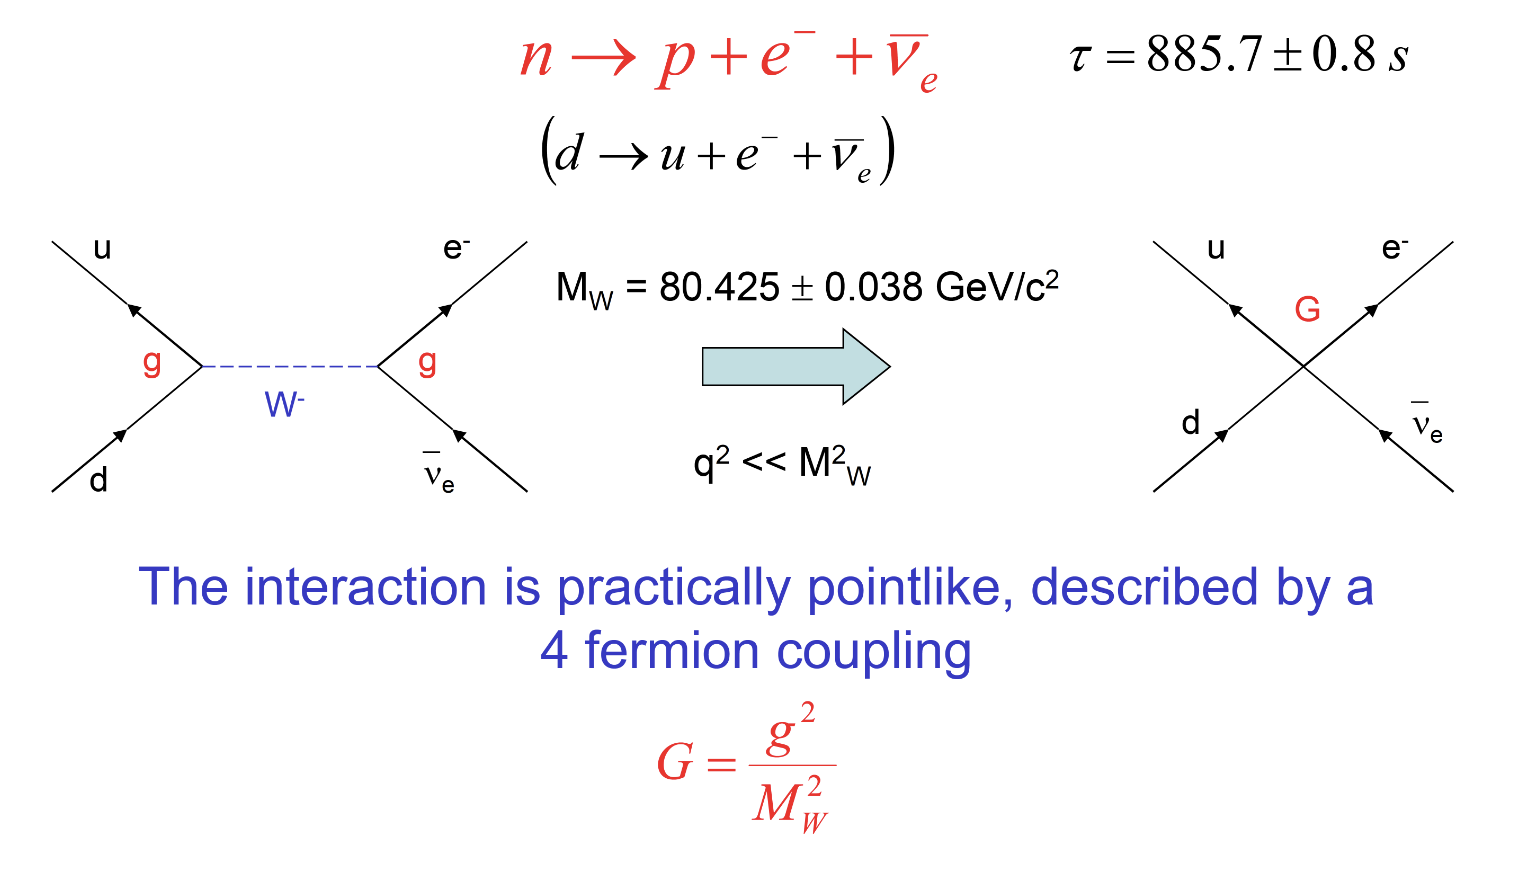
\includegraphics[height=7cm]{../figures/Fermi.png}
\end{frame}

% =================================================
\begin{frame}{Neutrino in the SM}
\begin{itemize}
  \item \textbf{Fermion masses:} generated via Yukawa couplings to the Higgs field,
  \[
  \mathcal{L}_Y = y \, \bar{\psi}_L H \psi_R + \text{h.c.}
  \]
  \item Requires \textbf{both left-handed and right-handed fields}
  \item \textbf{Left-handed neutrinos} $\nu_L$ only; no \textbf{right-handed neutrinos} $\nu_R$
  \item A \textbf{Dirac mass term} $m_D (\bar{\psi}_L \psi_R + \bar{\psi}_R \psi_L)$ \textbf{cannot be written}
  \item A \textbf{Majorana mass term} $m \, \psi_L^T C \psi_L$  also \textbf{forbidden by SM gauge symmetry}
\end{itemize}

\vspace{0.3cm}

\textbf{Conclusion:}
\[
\text{No allowed mass term} \;\Rightarrow\; m_\nu = 0 \quad \text{in the Standard Model.}
\]

\end{frame}

% =================================================
\section{Detection}

% =================================================
\begin{frame}{Typical neutrino sources:}
\begin{columns}
\begin{column}{0.4\textwidth}
\begin{itemize}
  \item The Sun \\
  (solar neutrinos)
  \item The atmosphere (atmospheric neutrinos)
  \item Nuclear reactors \\
  (reactor neutrinos)
  \item Particle accelerators (beam neutrinos)
\end{itemize}
\end{column}
\begin{column}{0.6\textwidth}
\centering
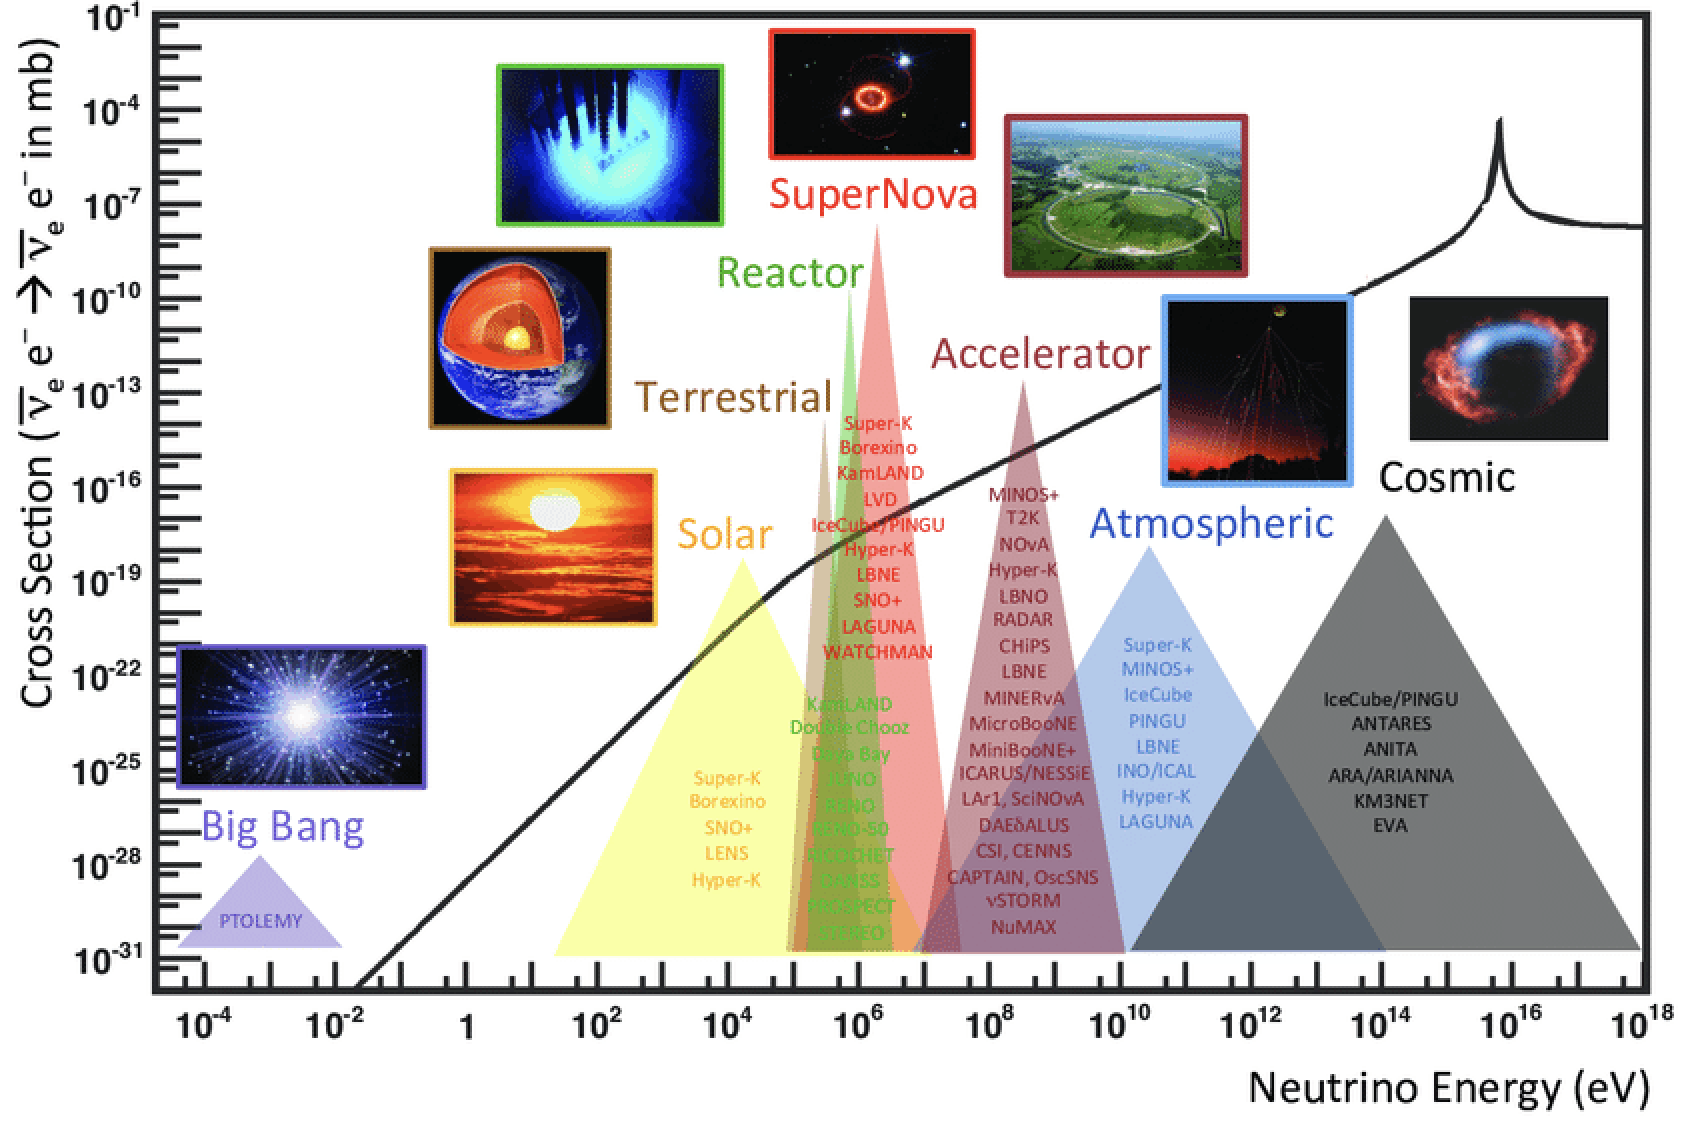
\includegraphics[width=\textwidth]{../figures/neutrinos.png}
\end{column}
\end{columns}

\vspace{0.3cm}

\textbf{Examples of experiments:} Super-Kamiokande, SNO, KamLAND, Daya Bay, T2K, NOvA, ...
\end{frame}

% =================================================
\begin{frame}{First Detection of the Neutrino (Cowan--Reines, 1956)}
\begin{columns}
    \column{0.7\textwidth}
    \textbf{Experimental idea:}
    \begin{itemize}
        \item A \textbf{nuclear reactor} as an intense source of electron antineutrinos $\bar{\nu}_e$
        \item Detector: water + cadmium chloride
        \item Detection via \textbf{inverse beta decay}:
        \[
        \bar{\nu}_e + p \;\to\; e^+ + n
        \]
        \end{itemize}

    \textbf{Detection signature (``delayed coincidence''):}
    \centering
    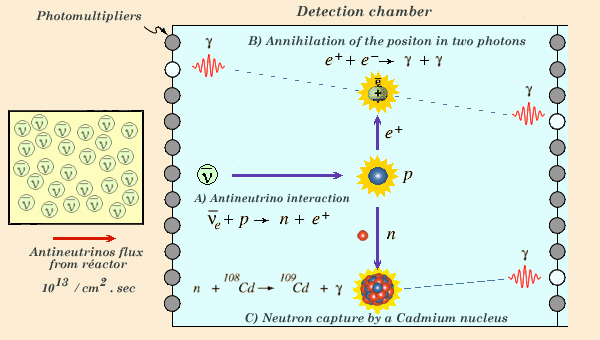
\includegraphics[height=3.5cm]{../figures/PrincipeExpCowan_En.jpg}
%    \begin{itemize}
%        \item $e^+$ annihilates $\to$ two gamma rays (prompt signal)
%        \item Neutron captured by Cd a few $\mu$s later $\to$ gamma ray (delayed signal)
%        \item This coincidence strongly suppresses background
%    \end{itemize}

    \column{0.3\textwidth}
    \centering
    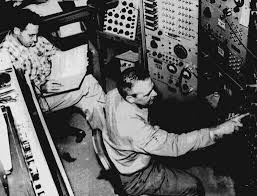
\includegraphics[height=2.5cm]{../figures/RC1.jpeg}
    \vspace{0.3cm}
    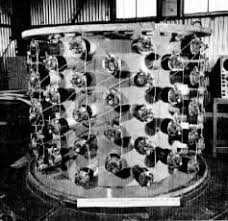
\includegraphics[height=3cm]{../figures/RC2.jpeg}
\end{columns}
\end{frame}
% =================================================
\section{Neutrino Oscillations: Theory}

% =================================================
\begin{frame}{Flavor Oscillation}
\centering
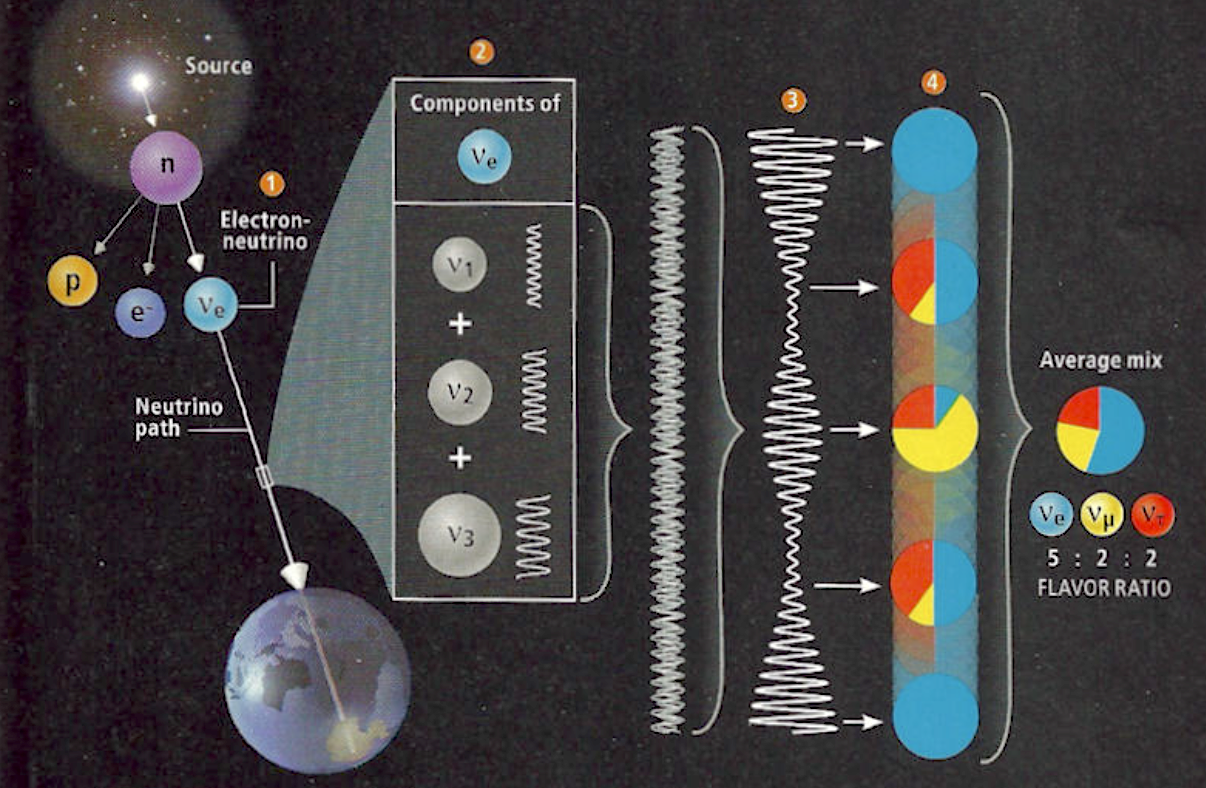
\includegraphics[height=7cm]{../figures/oscillation_.png}
\end{frame}

% =================================================
\begin{frame}{Detection}
\textbf{Basic experimental idea:}
\begin{itemize}
  \item Production of neutrinos with a known flavor
  \item Propagation over a baseline distance $L$
  \item Detection and flavor identification
  \item Search for flavor transitions
\end{itemize}

\vspace{0.3cm}

\textbf{Experimental signatures:}
\begin{itemize}
  \item \textbf{Disappearance:} deficit of the initial flavor
  \item \textbf{Appearance:} observation of a different flavor
  \item Characteristic dependence on
  \[
  \frac{L}{E}
  \]
  where $L$ is the baseline and $E$ is the neutrino energy
\end{itemize}
\end{frame}
% =================================================
\begin{frame}{The Idea of Mixing}

\textbf{Two-flavor approximation:}

\[
\begin{pmatrix}
\nu_e\\
\nu_\mu
\end{pmatrix}
=
\begin{pmatrix}
\cos\theta & \sin\theta\\
-\sin\theta & \cos\theta
\end{pmatrix}
\begin{pmatrix}
\nu_1\\
\nu_2
\end{pmatrix}
\]

\begin{itemize}
    \item $\theta$ : mixing angle
    \item $\theta = 0^\circ$ : no mixing, no oscillation
    \item $\theta = 45^\circ$ : maximal mixing
\end{itemize}

\[
|\nu_e\rangle
=
\cos\theta\,|\nu_1\rangle
+
\sin\theta\,|\nu_2\rangle
\]

\[
|\nu_\mu\rangle
=
-\sin\theta\,|\nu_1\rangle
+
\cos\theta\,|\nu_2\rangle
\]

\begin{itemize}
    \item Flavor eigenstates: $|\nu_e\rangle,\ |\nu_\mu\rangle$
    \item Mass eigenstates: $|\nu_1\rangle,\ |\nu_2\rangle$
    \item Flavor state = superposition of mass states
\end{itemize}

\end{frame}

\begin{frame}{Time Evolution}
Mass eigenstates propagate with different phases:
\[
|\nu_i(t)\rangle
=
e^{-iE_it}
|\nu_i\rangle
\]
An electron neutrino produced at $t=0$:
\[
|\nu(0)\rangle
=
|\nu_e\rangle
=
\cos\theta |\nu_1\rangle
+
\sin\theta |\nu_2\rangle
\]
After time $t$:
\[
|\nu(t)\rangle
=
\cos\theta\,e^{-iE_1t}|\nu_1\rangle
+
\sin\theta\,e^{-iE_2t}|\nu_2\rangle
\]


\begin{itemize}
    \item Global phase $e^{-iE_1t}$: unobservable
    \item Relative phase:
    \[
    \Delta\phi=(E_2-E_1)t
    \]
    \item Relative phase $\rightarrow$ quantum interference
    \item Quantum interference $\rightarrow$ flavor oscillation
\end{itemize}
\end{frame}

\begin{frame}{Deriving Oscillations}
Probability amplitude for detecting a muon neutrino:
\[
\mathcal{A}(\nu_e\rightarrow\nu_\mu)
=
\langle\nu_\mu|\nu(t)\rangle
\]
Using
\[
|\nu_\mu\rangle
=
-\sin\theta |\nu_1\rangle
+
\cos\theta |\nu_2\rangle
\]
gives
\[
\mathcal{A}
=
\sin\theta\cos\theta
\left(
e^{-iE_2t}
-
e^{-iE_1t}
\right)
\]
Therefore
\[
P(\nu_e\rightarrow\nu_\mu)
=
|\mathcal{A}|^2
\]
\[
=
\sin^2(2\theta)
\sin^2\left(
\frac{(E_2-E_1)t}{2}
\right)
\]
\end{frame}

\begin{frame}{Oscillation Probability}
For ultra-relativistic neutrinos:
\[
E_i
\approx
E+\frac{m_i^2}{2E}
\]
Therefore
\[
E_2-E_1
=
\frac{\Delta m^2}{2E}
\]
with
\[
\Delta m^2
=
m_2^2-m_1^2
\]
Using $t\approx L$:
\[
P(\nu_e\rightarrow\nu_\mu)
=
\sin^2(2\theta)
\sin^2\left(
\frac{\Delta m^2L}{4E}
\right)
\]

\vspace{0.3cm}
\textbf{Three ingredients for oscillations:}
\begin{itemize}
\item Mixing ($\theta\neq0$)
\item Different masses ($\Delta m^2\neq0$)
\item Ratio $L/E$
\end{itemize}
\end{frame}

\begin{frame}{The PMNS (Pontecorvo-Maki-Nakagawa-Sakata) Matrix}
Real neutrinos exist in three flavors:$\nu_e,\; \nu_\mu,\; \nu_\tau$

The mixing is described by the PMNS matrix:
\[
|\nu_\alpha\rangle
=
\sum_{i=1}^{3}
U_{\alpha i}
|\nu_i\rangle
\]

\begin{itemize}
    \item $\alpha=e,\mu,\tau$ (flavor)
    \item $i=1,2,3$ (mass)
    \item $U$ is a $3\times3$ unitary matrix
\end{itemize}

\textbf{The change of basis between flavor and mass eigenstates}
Parameterization:

\begin{center}
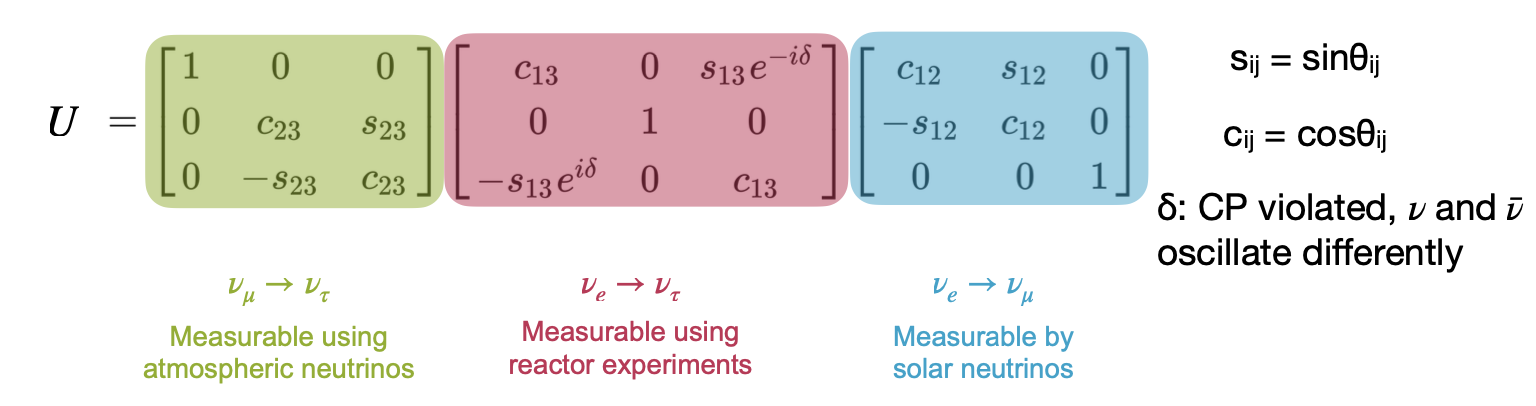
\includegraphics[height=3cm]{../figures/PMNS.png}
\end{center}
\end{frame}

\begin{frame}{Parameters of the PMNS Matrix}

Experiments measure the parameters of $U$:
\begin{itemize}
    \item Mixing angles:
    \[
    \theta_{12},\;
    \theta_{23},\;
    \theta_{13}
    \]

    \item CP-violating phase:
    \[
    \delta_{\rm CP}
    \]

    \item Mass-squared differences:
    \[
    \Delta m^2_{21},
    \qquad
    \Delta m^2_{31}
    \]
\end{itemize}

\centering

\includegraphics[height=3cm]{../figures/changing.jpg}
\end{frame}

% =================================================
\section{Neutrino Oscillations: Experiment}
% ===================== SUPER-KAMIOKANDE =====================
\begin{frame}{Super-Kamiokande: Motivation}
\begin{columns}
\begin{column}{0.52\textwidth}
\textbf{Primary Motivation: Proton Decay Search}
\begin{itemize}
  \item Successor to Kamiokande (10$\times$ larger volume)
  \item Test Grand Unified Theories (GUTs)
  \item Push proton lifetime limits
\end{itemize}

\vspace{0.3cm}

\textbf{Additional Physics Goals}
\begin{itemize}
  \item Atmospheric neutrino oscillations
  \item Solar neutrinos (resolve Solar Neutrino Problem)
  \item Supernova neutrino bursts
  \item Astrophysical neutrinos
\end{itemize}
\end{column}

\begin{column}{0.48\textwidth}
\centering
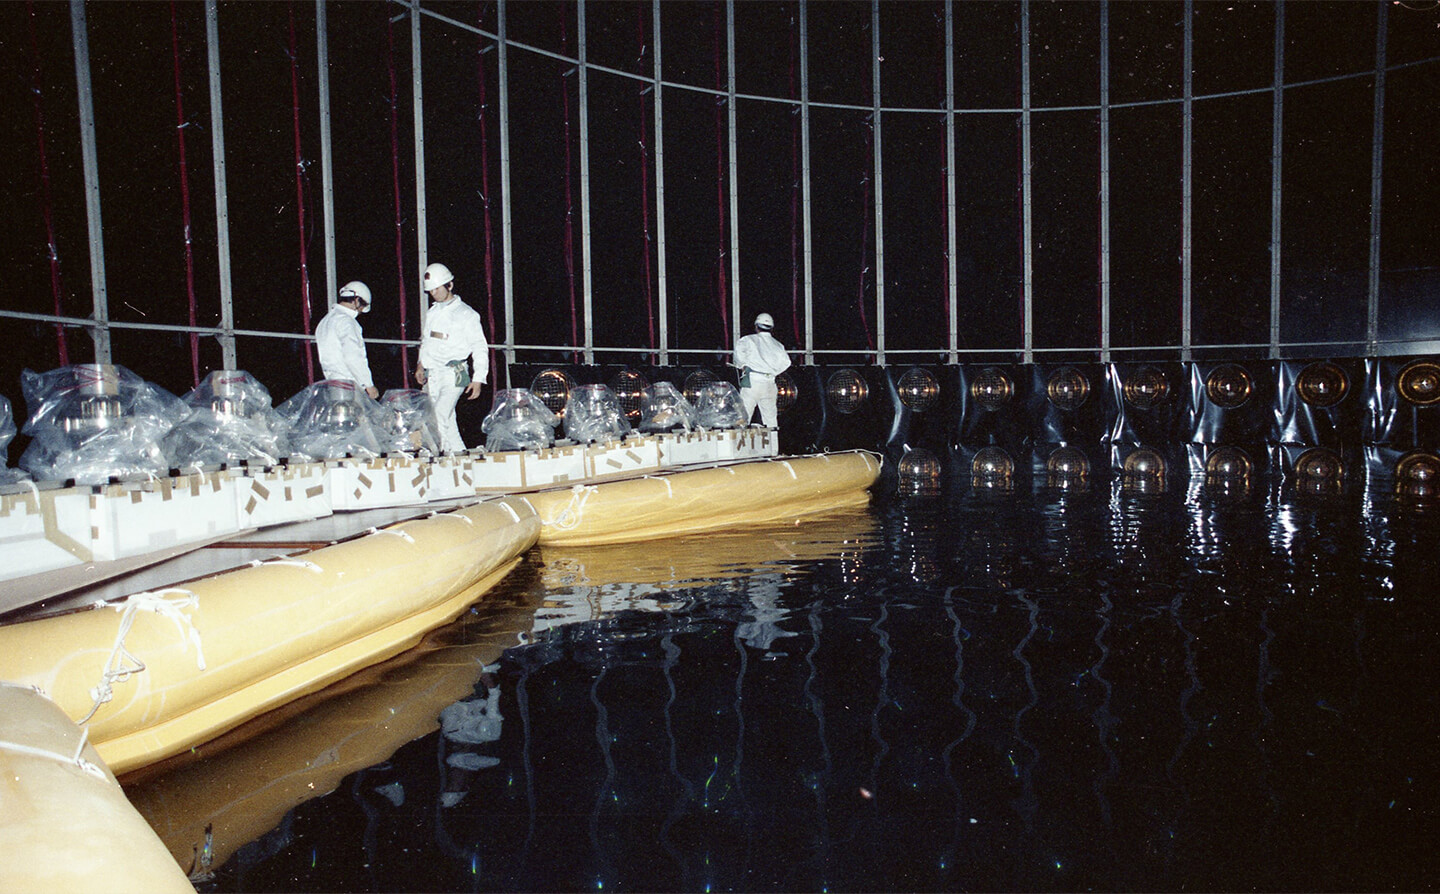
\includegraphics[width=\textwidth]{../figures/ka.jpg}

\vspace{0.3cm}

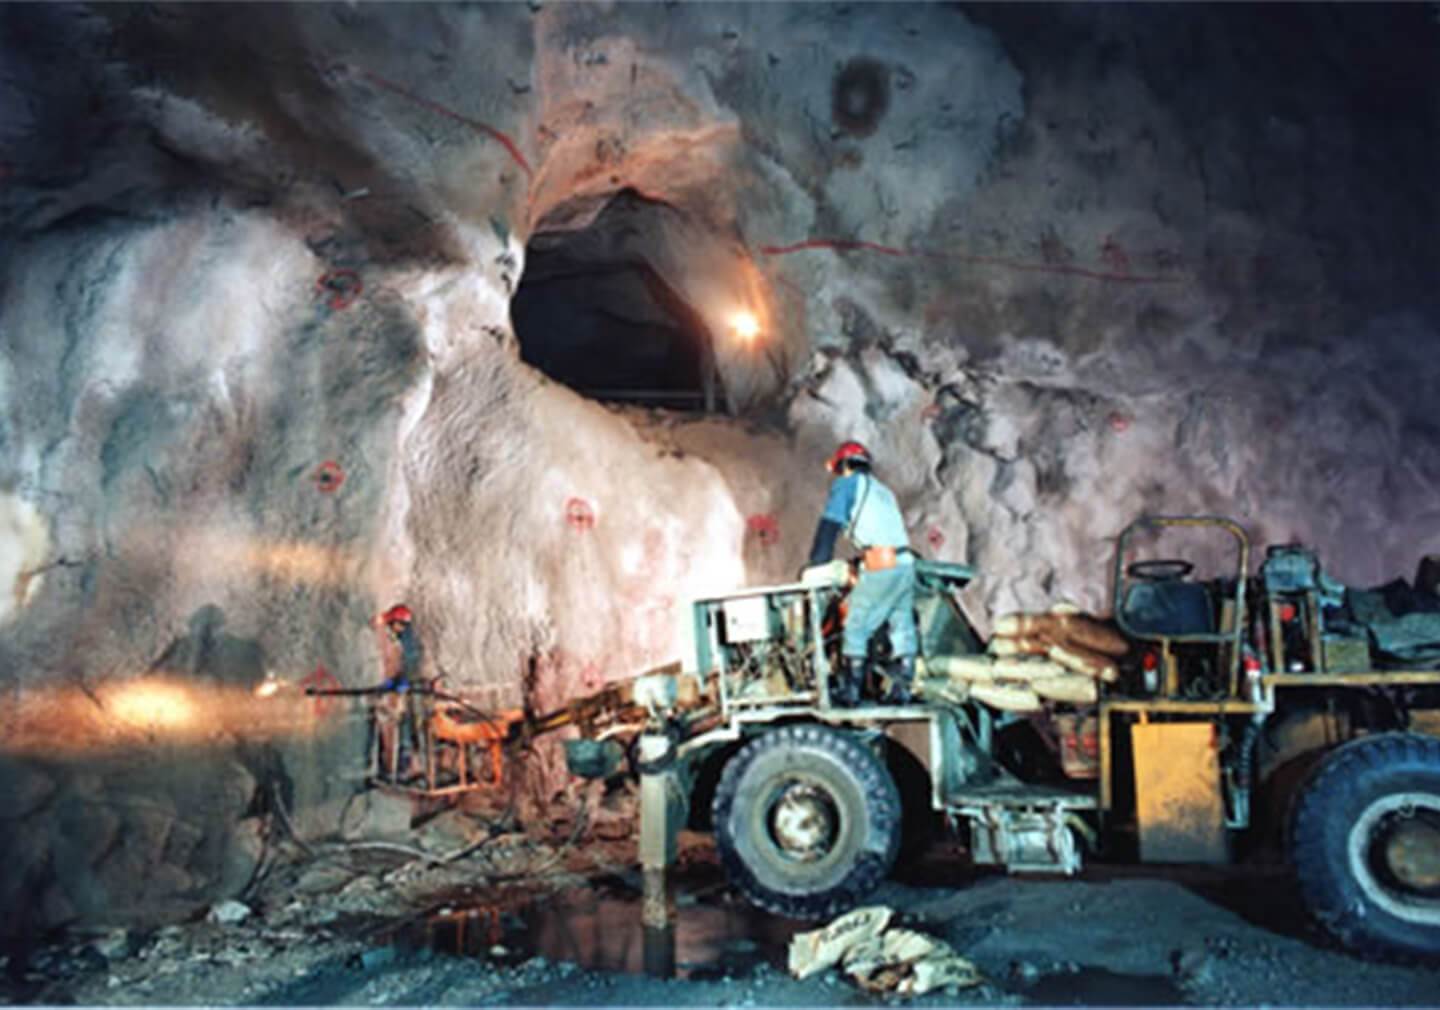
\includegraphics[width=\textwidth]{../figures/su.jpg}
\end{column}
\end{columns}
\end{frame}

\begin{frame}{Atmospheric Neutrinos}
\begin{itemize}
    \item Produced by cosmic-ray interactions in upper atmosphere: \[\pi^{\pm} \to \mu^{\pm} + \nu_{\mu} \, (\bar{\nu}_{\mu}) \qquad \mu^{\pm} \to e^{\pm} + \nu_{e} \, (\bar{\nu}_{e}) + \bar{\nu}_{\mu} \, (\nu_{\mu})\]
    \item Dominant $\nu_\mu$ component; expected $\nu_\mu / \nu_e$ ratio $\approx 2$
    \item Detected as e-like (fuzzy) and $\mu$-like (sharp) Cherenkov rings in water
\end{itemize}

    \begin{columns}
        \column{0.5\textwidth}
        \centering
        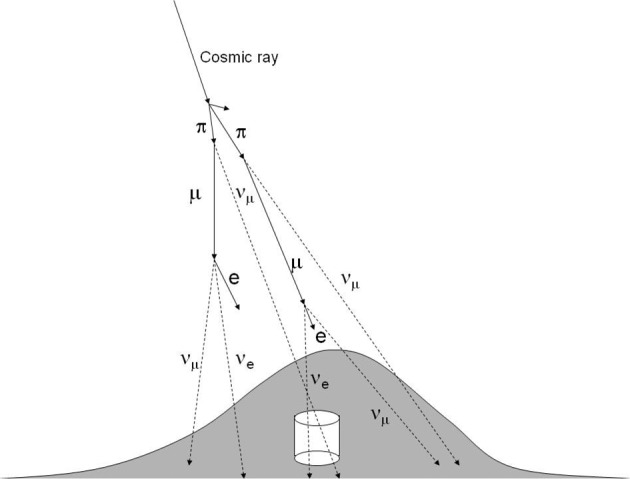
\includegraphics[width=0.9\textwidth]{../figures/cosmic-ray-atmospheric-neutrino-generation.jpg}
        \column{0.5\textwidth}
        \centering
        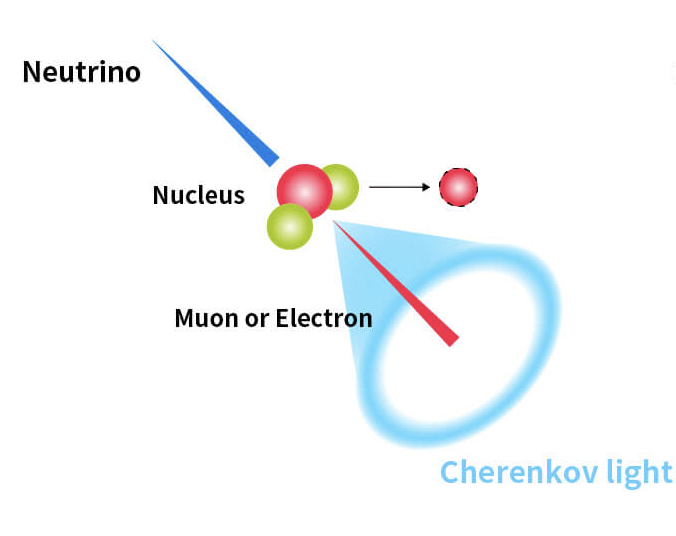
\includegraphics[width=0.9\textwidth]{../figures/Screenshot 2026-06-16 at 01.02.24.png}
    \end{columns}
\end{frame}

\begin{frame}{Super-Kamiokande}
\begin{itemize}
    \item 50\,kt ultra-pure water Cherenkov detector in Kamioka Mine, Japan
    \item 1\,km underground ($\sim$2.7\,km water equivalent overburden)
    \item $\sim$11,000 20-inch photomultiplier tubes (PMTs)
    \item Data taking started in 1996 (led by Takaaki Kajita)
\end{itemize}

\vspace{1cm}
    \begin{columns}
        \column{0.5\textwidth}
        \centering
        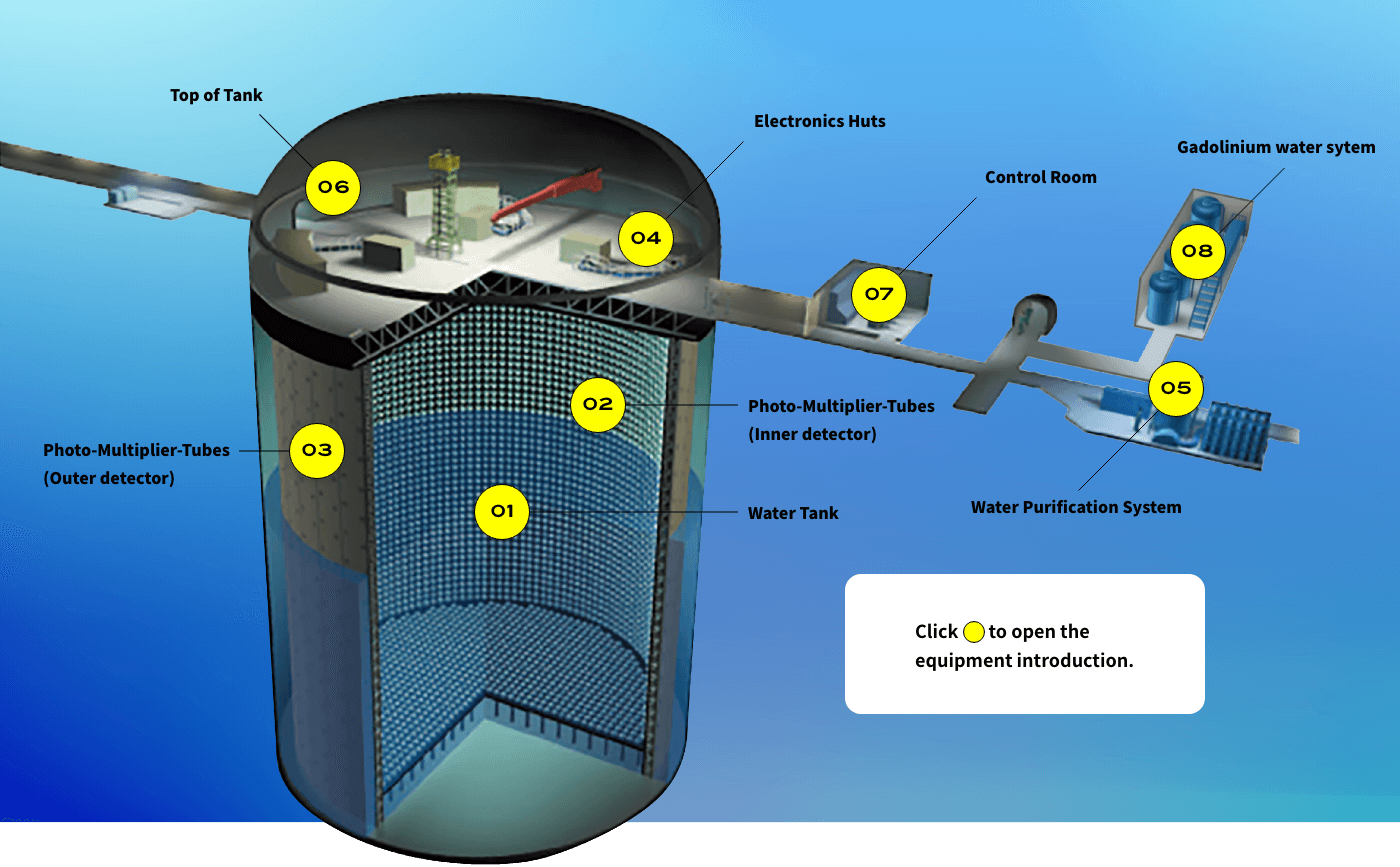
\includegraphics[width=0.9\textwidth]{../figures/detector_main.png}
        \column{0.5\textwidth}
        \centering
        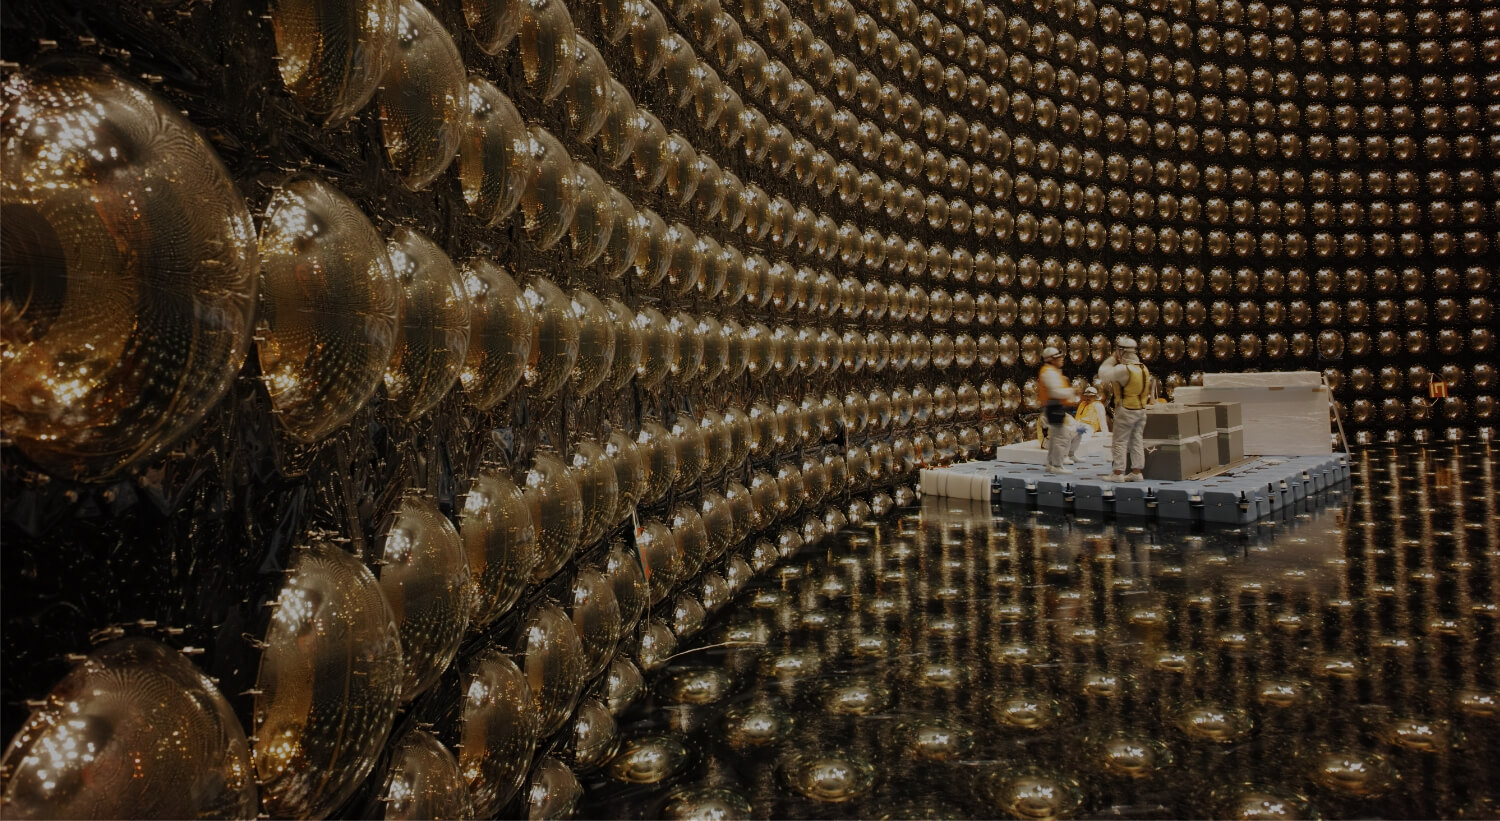
\includegraphics[width=0.9\textwidth]{../figures/sk_hero_01.jpg}
    \end{columns}
\end{frame}

\begin{frame}{Super-Kamiokande}
$\nu_\mu + n \rightarrow \mu^- + p$
    \begin{center}
        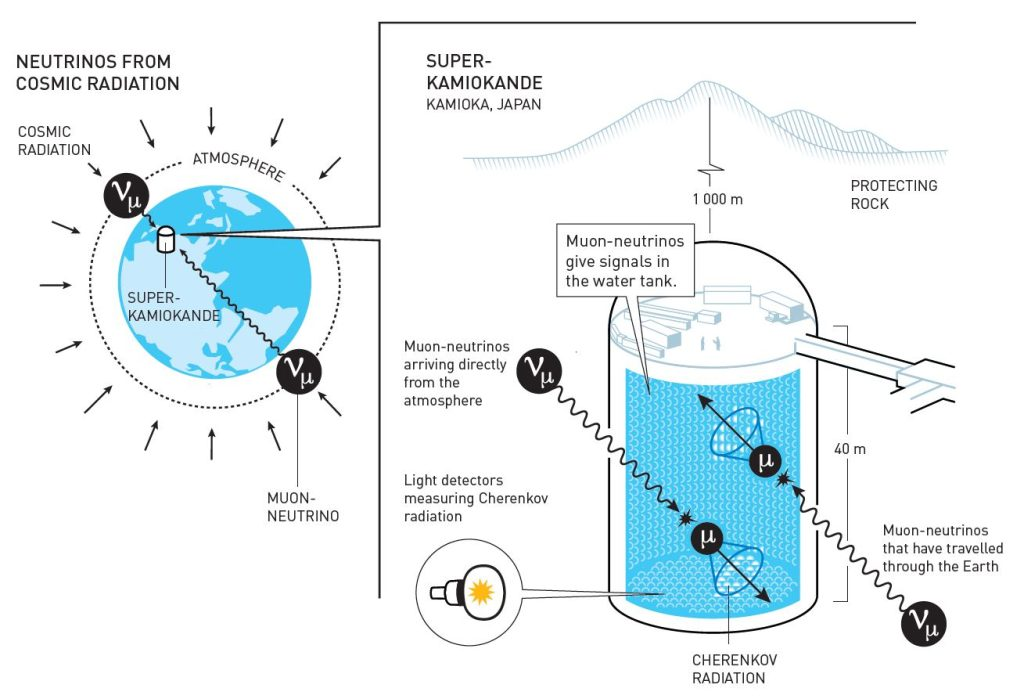
\includegraphics[width=0.85\textwidth]{../figures/super-k.jpeg}
    \end{center}

\end{frame}

\begin{frame}{Zenith Angle Distribution}
\begin{itemize}
    \item Downward events ($\cos\theta_z \approx +1$): short baseline ($\sim$20\,km)
    \item Upward events ($\cos\theta_z \approx -1$): long baseline through Earth ($\sim$13,000\,km)
    \item Strong deficit in upward-going $\mu$-like events
    \item e-like events consistent with no-oscillation expectation
    \item Classified by energy: sub-GeV and multi-GeV events
\end{itemize}
    \centering
    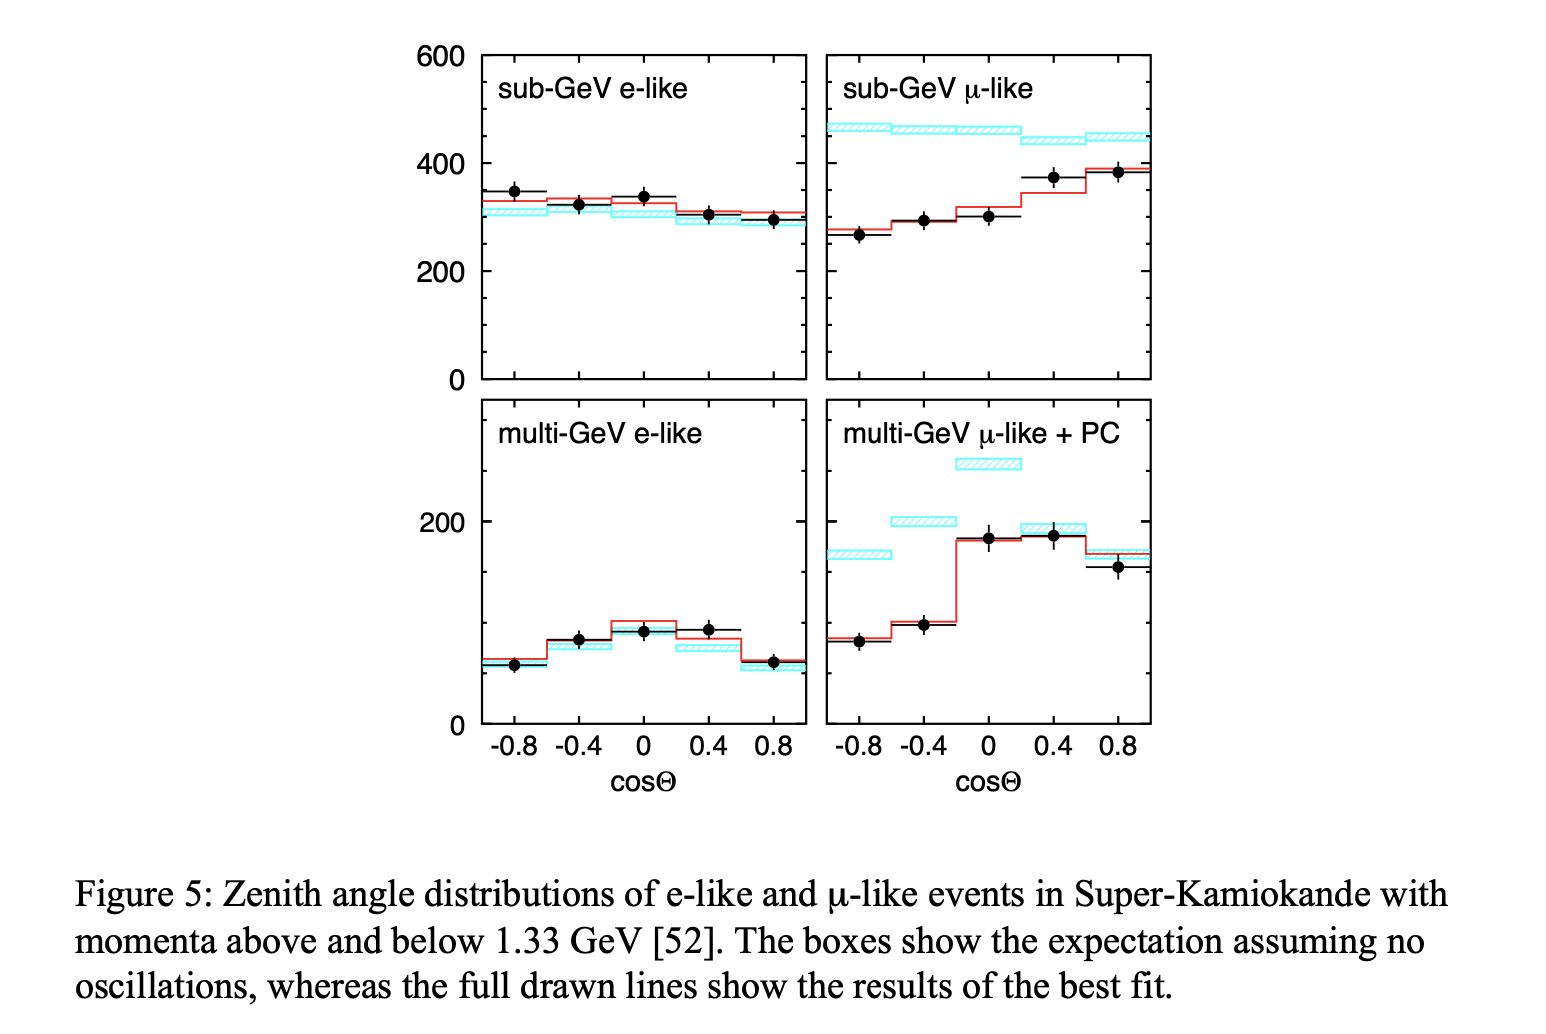
\includegraphics[width=0.83\textwidth]{../figures/zenith.png}
    
\begin{textblock*}{2cm}(2.9cm,4.5cm)
    \rotatebox{90}{\tiny number of events}
\end{textblock*}
\end{frame}

\begin{frame}{Super-K Results}
    \begin{itemize}
    \item Observed $\mu$-like flux $\sim$50\% less than expected for upward events ($\gtrsim 5\sigma$)
    \item Best-fit: $\Delta m^2_{32} \approx 2.5 \times 10^{-3}$\,eV$^2$, $\sin^2 2\theta_{23} \approx 1$ \\ (near-maximal mixing) $\Rightarrow \Delta m^2_{32} \neq 0,  \theta_{23} \approx 45^\circ$
    \item Evidence for $\nu_\mu \to \nu_\tau$ oscillations (disappearance channel)
    \item Confirmed by long-baseline experiments (K2K) later
\end{itemize}

    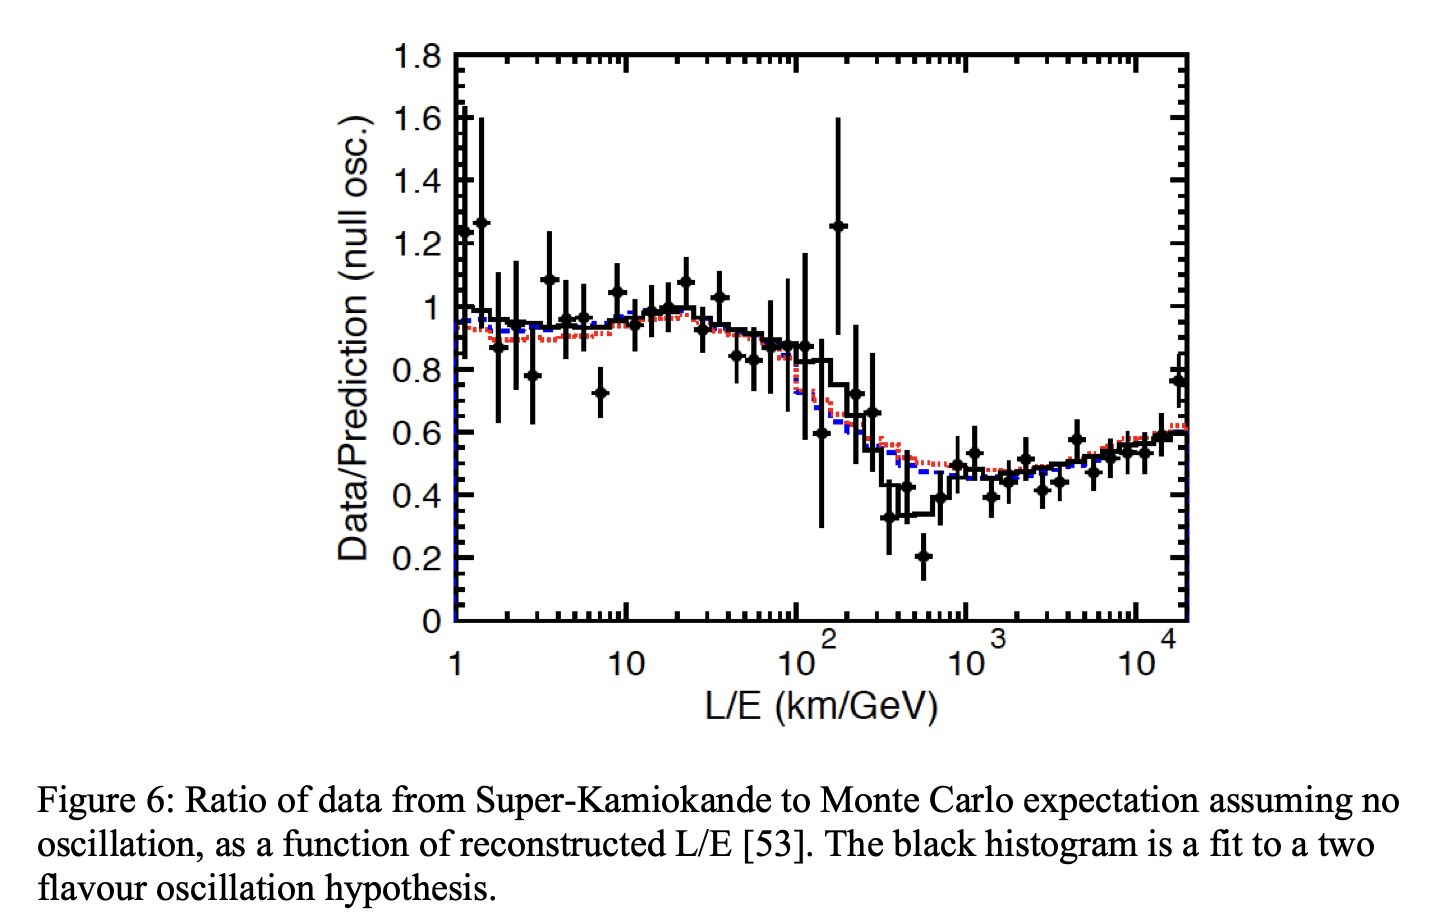
\includegraphics[width=0.9\textwidth]{../figures/MC.png}
\end{frame}

\begin{frame}{Why Atmospheric Neutrinos?}


\textbf{GeV energy spectrum}
    \begin{itemize}
        \item Consistent with atmospheric neutrino production
        \item Too energetic to be solar neutrinos
        \item Astrophysical neutrino contribution negligible in this energy range
    \end{itemize}

\textbf{Nearly isotropic arrival directions}
    \begin{itemize}
        \item Expected from production throughout Earth's atmosphere
    \end{itemize}

\textbf{Expected $\nu_e$ rate}
    \begin{itemize}
        \item Agrees with atmospheric neutrino flux predictions
    \end{itemize}

\textbf{$L/E$-dependent $\nu_\mu$ disappearance}
    \begin{itemize}
        \item Signature of atmospheric neutrino oscillations
    \end{itemize}


\end{frame}

% ===================== SNO =====================
\begin{frame}{The Solar Neutrino Problem \& SNO Motivation}
\textbf{The Solar Neutrino Problem}
\begin{itemize}
    \item Standard Solar Model predicts high $\nu_e$ flux from pp-chain fusion
    \item Main reaction: $p + p \to {}^2\mathrm{H} + e^+ + \nu_e$
    \item Experiments (Homestake, GALLEX, Super-K, ...) measured only $\sim 1/3$ of expected $\nu_e$
    \item Persistent discrepancy for $\sim$35 years (1968--2002)
\end{itemize}

\vspace{0.3cm}

\textbf{SNO}
\begin{itemize}
    \item Test if deficit was due to solar model or neutrino oscillations
    \item Distinguish $\nu_e$ flux vs total neutrino flux (all flavors)
    \item Confirm $\nu_e \to \nu_{\mu/\tau}$ oscillations
\end{itemize}
\end{frame}

\begin{frame}{SNO Detection Channels}
\begin{columns}
    \column{0.5\textwidth}
    \begin{itemize}
        \item Charged Current (CC): $\nu_e + d \to p + p + e^-$ \\
        (sensitive only to $\nu_e$)
        \vspace{2.5em}
        \item Neutral Current (NC): $\nu_x + d \to p + n + \nu_x$ \\
        (equal sensitivity to all flavors)
        \vspace{2.5em}
        \item Elastic Scattering (ES): $\nu_x + e^- \to \nu_x + e^-$ \\
        (all flavors, $\nu_e$ enhanced)
    \end{itemize}
    
    \column{0.5\textwidth}
        \centering
        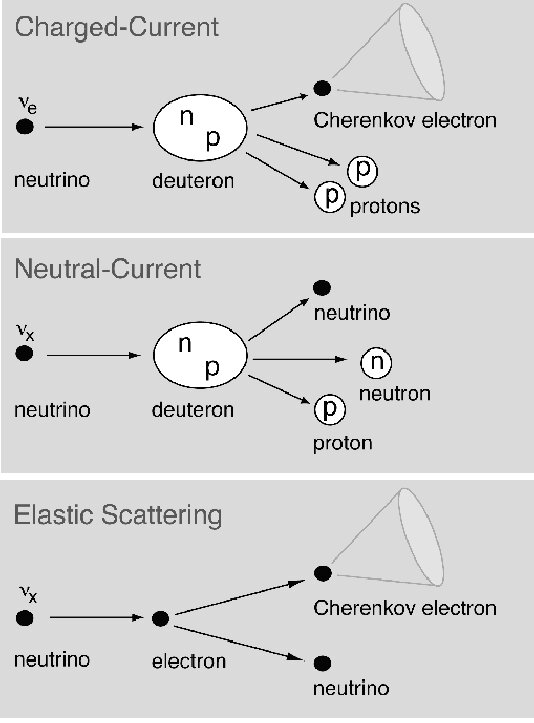
\includegraphics[width=0.9\textwidth]{../figures/CC-NC-ES-reactions-in-SNO_W640.jpg}
    \end{columns}
    
\end{frame}

\begin{frame}{Detection}
\centering
    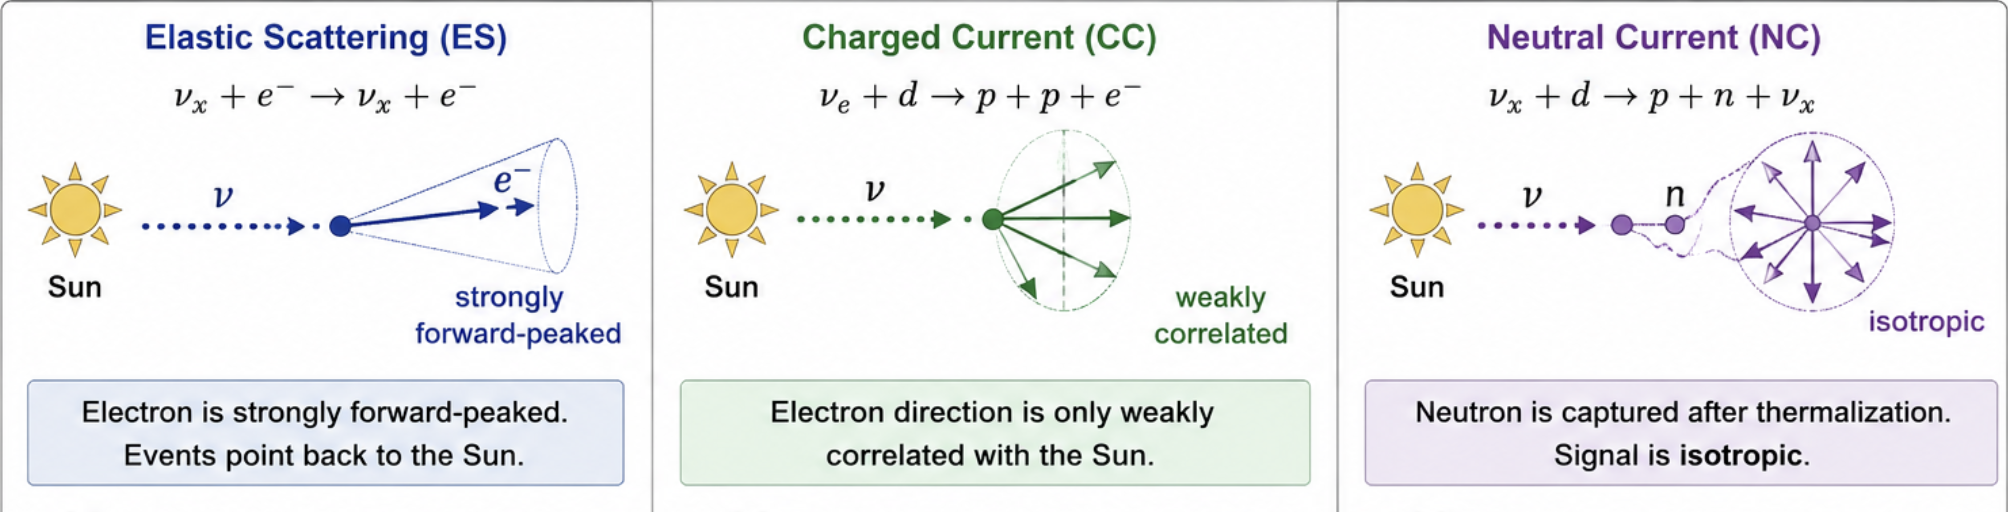
\includegraphics[width=0.95\textwidth]{../figures/123.png}
    \vspace{1em}
    \begin{itemize}
        \item Both CC and ES interactions produce an electron:
        \item Both electrons emit Cherenkov light $\Rightarrow$ cannot be distinguished event-by-event
        \item Separation performed \textbf{statistically} using the angle $\theta_\odot$ between the reconstructed electron direction and the Sun
        \item The NC channel is a bit more complicated
    \end{itemize}
\end{frame}

\begin{frame}{NC Detection in SNO}

\textbf{Reaction:}
\[
\nu_x + d \rightarrow p + n + \nu_x
\]

\begin{itemize}
    \item Sensitive to all flavors: $\nu_e, \nu_\mu, \nu_\tau$
    \item Only observable product: \textbf{free neutron}
\end{itemize}

\vspace{0.3cm}
\textbf{Detection strategy: neutron capture}

\begin{itemize}
    \item Neutron thermalizes in heavy water ($\mathrm{D_2O}$)
    \item Captures on:\\
         Deuteron (Phase I): $n + d \rightarrow t + \gamma$ (6.25 MeV)\\
         Chlorine (Phase II, with NaCl): $n + {}^{35}\mathrm{Cl} \rightarrow {}^{36}\mathrm{Cl} + \gamma$ (8.6 MeV)
\end{itemize}

\textbf{Signal in detector:}
\[
\text{Neutron capture} \;\rightarrow\; \gamma \
\]


% --- image overlay (top right corner) ---
\begin{textblock*}{4cm}(8.5cm,1.2cm)
    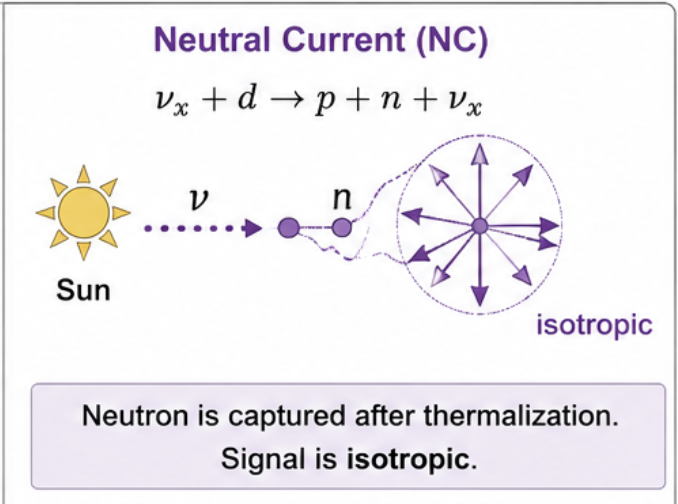
\includegraphics[width=4cm]{../figures/3.png}
\end{textblock*}

\end{frame}
\begin{frame}{Sudbury Neutrino Observatory (SNO)}
\begin{itemize}
    \item 1\,kt heavy water (D$_2$O) detector located 2\,km underground in Canada
    \item Arthur B. McDonald and collaboration (data 1999--2006)
    \item Unique sensitivity to all active neutrino flavors via deuterium reactions
    \item Heavy water allows neutral-current detection of $\nu_\mu$ and $\nu_\tau$
\end{itemize}

\begin{columns}
    \column{0.5\textwidth}
    \centering
    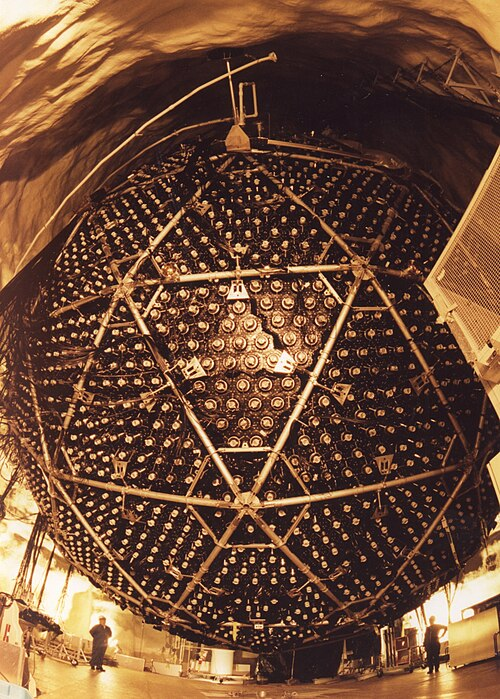
\includegraphics[width=0.75\textwidth]{../figures/Sudbury_Neutrino_Observatory.detector_outside.jpg}
    \column{0.5\textwidth}
    \centering
    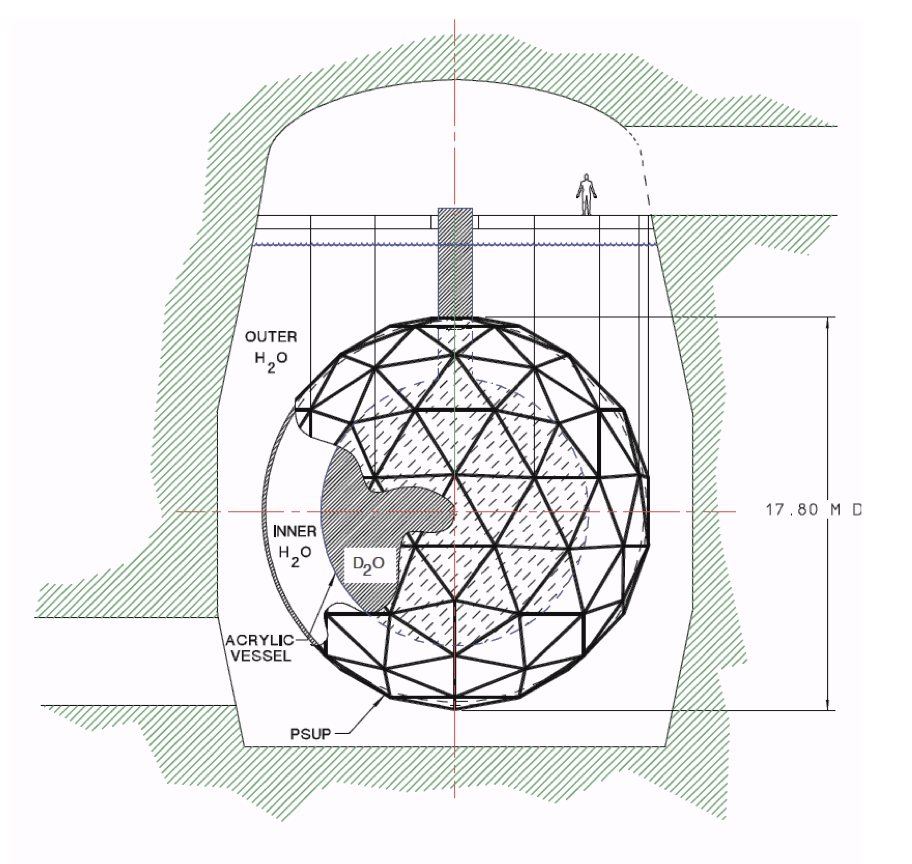
\includegraphics[width=0.85\textwidth]{../figures/sno_layout.png}
\end{columns}
\end{frame}

\begin{frame}{Sudbury Neutrino Observatory (SNO)}

\centering
        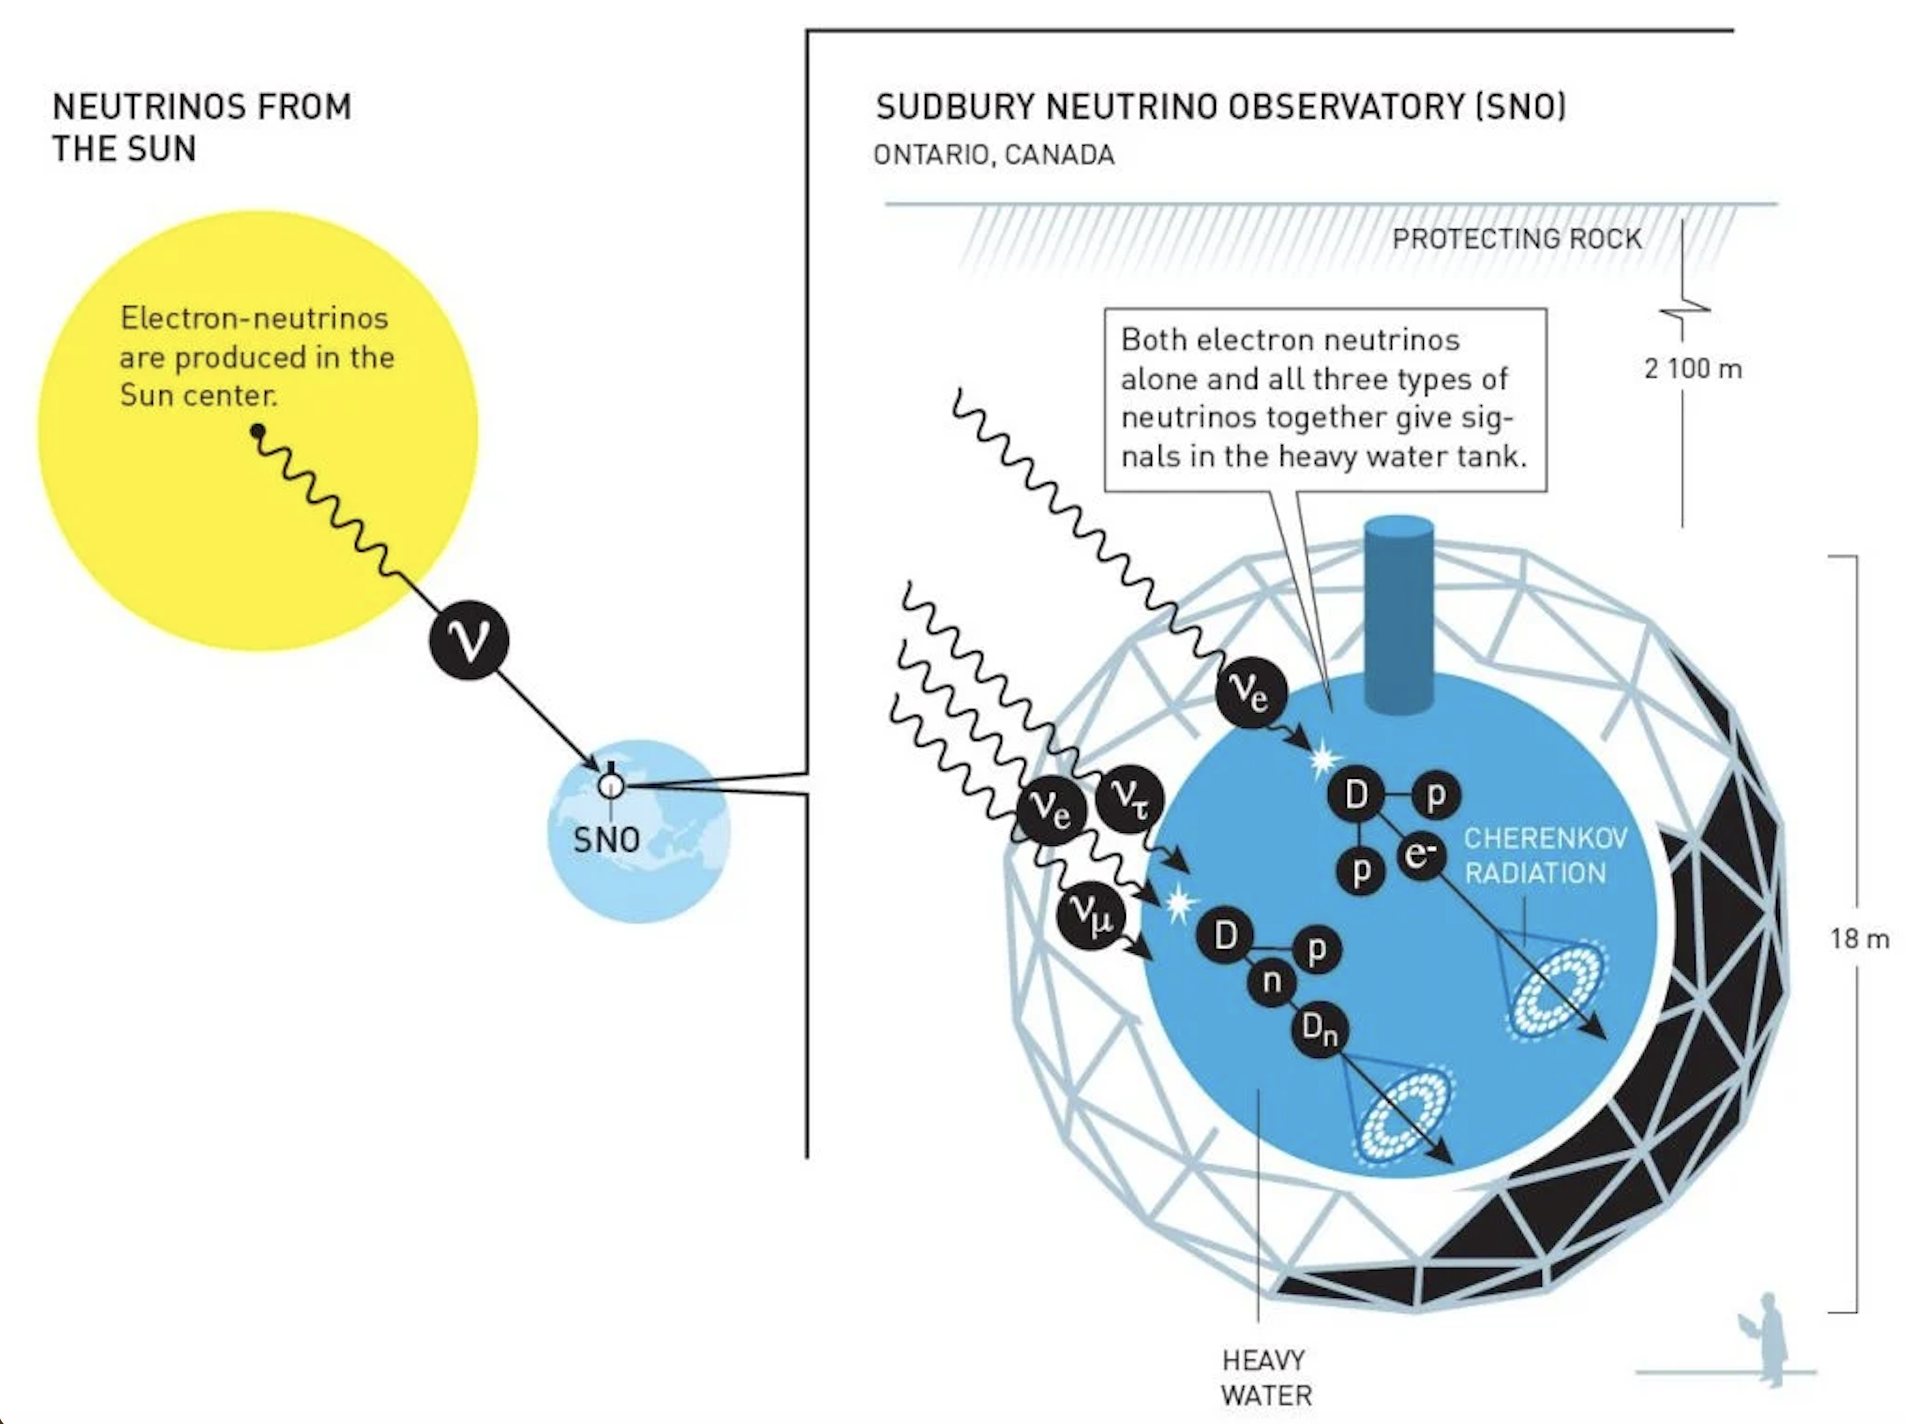
\includegraphics[width=0.9\textwidth]{../figures/sno.png}
\end{frame}

\begin{frame}{SNO Key Results}
\begin{itemize}
    \item CC flux significantly lower than Standard Solar Model (SSM) prediction
    \item NC flux agrees with SSM: total active neutrino flux matches expectations
    \item Only $\sim$1/3 of solar $\nu_e$ arrive as $\nu_e$; remaining 2/3 oscillated to $\nu_{\mu/\tau}$
    \item Confirmed solar neutrino oscillations
\end{itemize}

\centering
        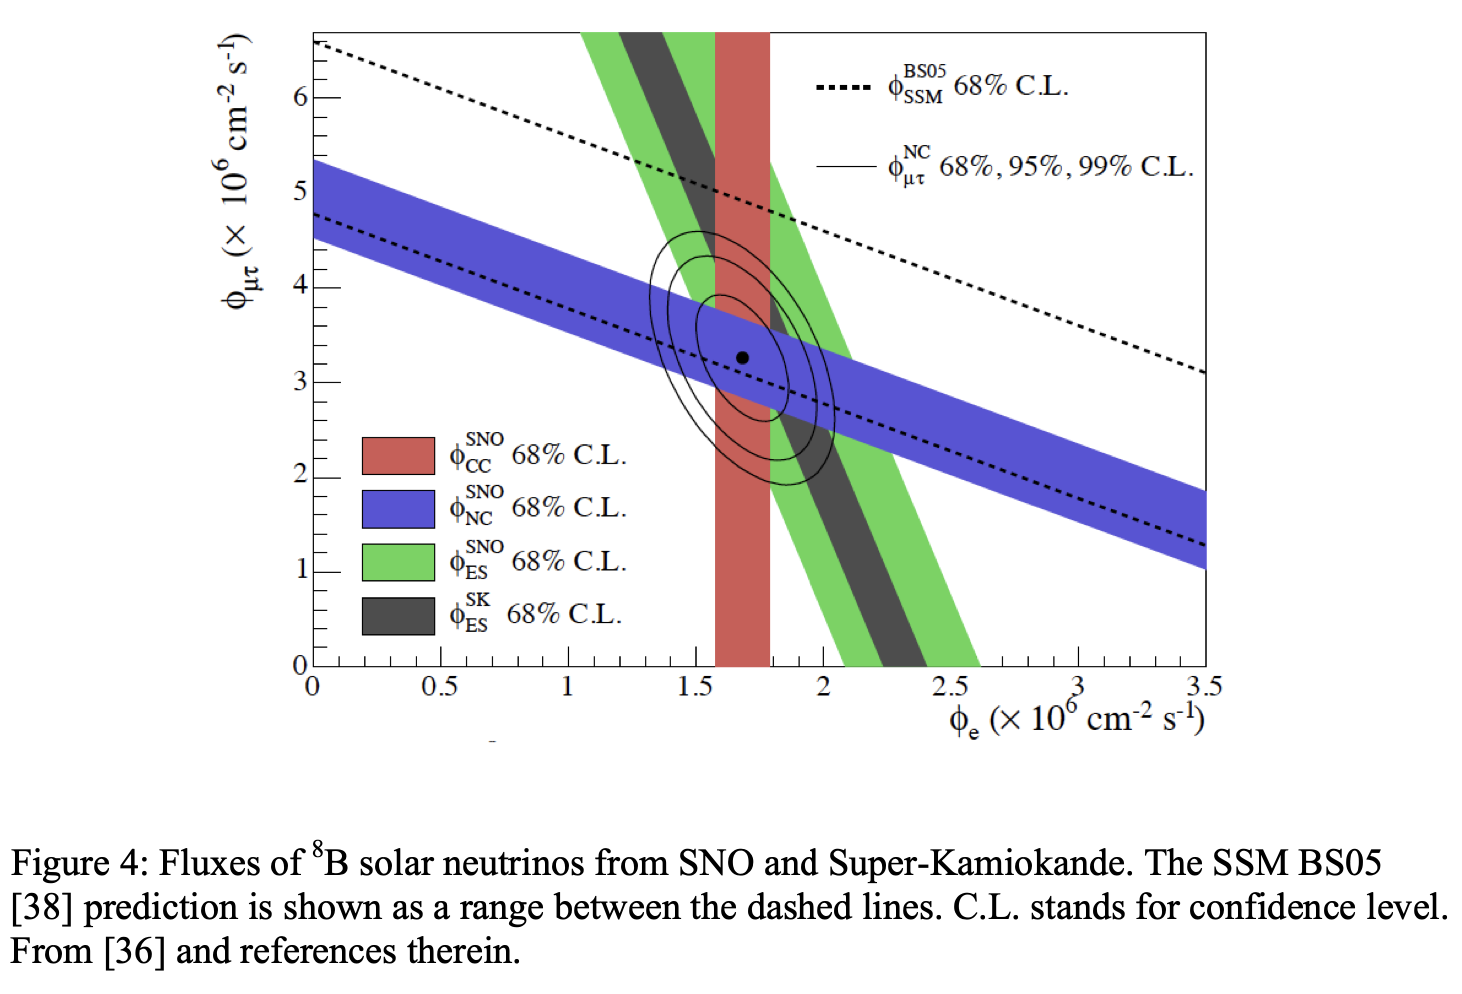
\includegraphics[width=0.85\textwidth]{../figures/fluxes.png}
\end{frame}

\begin{frame}{Why Solar Neutrinos?}

\textbf{Directionality}
    \begin{itemize}
        \item Strong peak in $\cos\theta_\odot \approx 1$
        \item Events point back to the Sun
    \end{itemize}

\textbf{Energy scale}
    \begin{itemize}
        \item MeV-scale events ($\lesssim 20\,\mathrm{MeV}$)
        \item Consistent with solar fusion neutrino spectrum
    \end{itemize}

\textbf{Time dependence}
    \begin{itemize}
        \item Signal follows Sun's position in the sky
    \end{itemize}

\textbf{Consistency check}
    \begin{itemize}
        \item NC flux matches solar model prediction
        \item CC deficit indicates flavor conversion
    \end{itemize}


\end{frame}

% ===================== SUMMARY =====================
\section{Summary}

\begin{frame}{Summary}
\begin{itemize}
    \item Clear observation of $\nu_\mu$ disappearance (Super-K) and $\nu_e \to \nu_{\mu/\tau}$ transitions (SNO)
    \item Super-K (atmospheric) + SNO (solar): definitive proof of neutrino oscillations
    \item Neutrino flavor change established; oscillation parameters well measured
    \item Neutrino oscillations $\Rightarrow$ masses $\Rightarrow$ BSM.
    \item Pauli (1930) $\to$ detection (1956) $\to$ oscillations (1998--2002).
    \item Major open questions remain: mass ordering, absolute masses, CP violation, Dirac vs Majorana.
\end{itemize}
\end{frame}


% =================================================
\begin{frame}[allowframebreaks]{References}
\footnotesize
\begin{itemize}
  \item \href{https://en.wikipedia.org/wiki/Beta_decay}{Beta decay}.
  \item \href{https://www.nobelprize.org/prizes/physics/1945/pauli/lecture/}{W. Pauli, Open Letter to the Group of Radioactive Ladies and Gentlemen (1930)}.
  \item \href{https://doi.org/10.1007/BF02959820}{E. Fermi, Tentativo di una teoria dell'emissione dei raggi $\beta$, Nuovo Cimento 11, 1--19 (1934)}
  \item \href{https://doi.org/10.1126/science.124.3212.103}{Cowan-Reines, Observation of the Free Neutrino, Science 124, 103 (1956)}
  \item \href{https://radioactivity.eu.com/articles/phenomenon/1956-neutrino-discovery}{Cowan--Reines, The Discovery of the Neutrino (1956)}
  \item \href{https://www.nobelprize.org/prizes/physics/2015}{Nobel Prize in Physics 2015}
  \item \href{https://universe-review.ca/R15-13-neutrino.htm}{The missing neutrinos}
  \item \href{https://pdg.lbl.gov/2024/reviews/rpp2024-rev-neutrino-mixing.pdf}{Particle Data Group, Review of Neutrino Mixing (2024--2025)}
  \item \href{https://www-sk.icrr.u-tokyo.ac.jp/en/sk/about/detector/}{Super Kamiokande}
  \item \href{https://www.researchgate.net/publication/232770047_Application_of_Signal_Processing_to_Investigate_the_Total_Active_8_B_Solar_Neutrino_Flux_Signal_from_Sudbury_Neutrino_Observatory_SNO}{Application of Signal Processing to Investigate the Total Active 8 B Solar Neutrino Flux Signal from Sudbury Neutrino Observatory (SNO)}
\end{itemize}
\end{frame}

\end{document}